% !TEX root = sum1.tex
\section{Problem Formulation}
In this section, we give the description of the problem, then present the deterministic and stochastic formalution.
% First, we will introduce some preliminary knowledge about our problem as follows.

\subsection{Problem Description}
% In this section we present the model that generates seat assignment under deterministic demands.

Consider a set of groups, each consisting of no more than $m$ people, to be assigned to a set of seats. These groups are denoted by a demand vector, $\mathbf{d} = (d_1, \ldots, d_m)$. Each element, $d_i, 1 \leq i \leq m$, indicates the number of group type $i$ containing $i$ people. For illustration, we consider the layout as $N$ rows, each row with $S_{j}$ seats, $j = 1, \ldots, N$. 

% Let the $i-$th group type contain $i$ people. 
% $(d_1, d_2, d_3, d_4) = (3,5,7,6)$

% But our model and formulation allow for a more general layout of the seats. 
According to the epidemic prevention requirements, the customers from the same group can sit together, while different groups should sit with social distancing. 
Suppose that each group has to leave one seat to maintain social distancing from the adjacent groups and different rows have no effect on each other, i.e., a person from one group can sit directly behind a person from another group.

% Considering the actual situation, social distancing is one seat in our paper 
To simplify the social distancing in the seat assignment, we add one to the original size of each group as the new size of the group and one dummy seat to each row. Take $s_{i} = i + 1$, $L_{j} = S_{j} +1$, $s_{i}$ is the new size of group type $i$ and $L_{j}$ is the length of row $j$.

Then we can illustrate the seat assignment for one row below. 

\begin{figure}[ht]
    \centering
    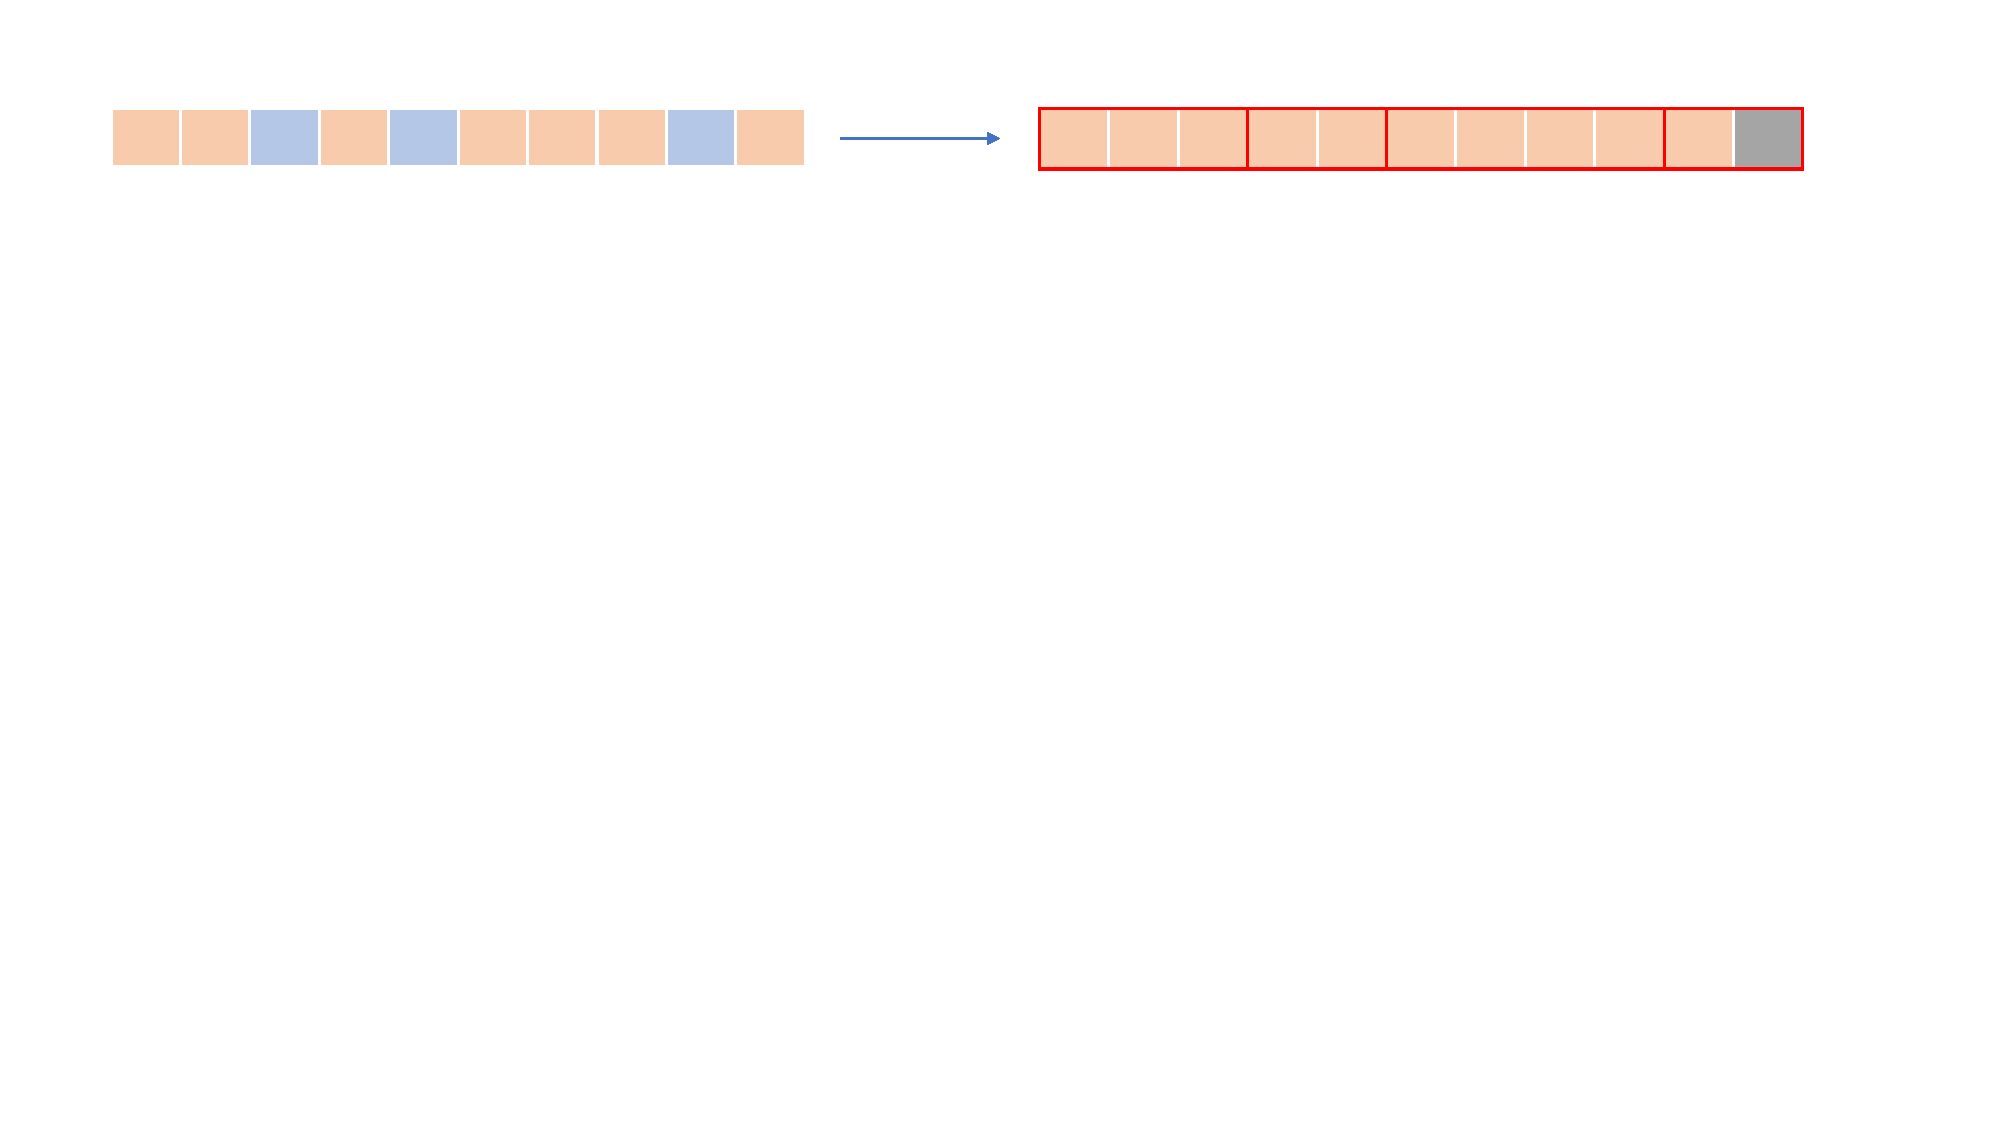
\includegraphics[width = 0.8\textwidth]{./Figures/dummy_seat.pdf}
    \caption{Problem Conversion}
\end{figure}

On the left side, the blue squares stand for the empty seats as the social distancing. The orange squares represent the seats sat by the groups. 
On the right side, one dummy seat is added at the end of the row. The orange squares surrounded by the red line are the seats taken by groups. Here, this row is placed two group of 1, one group of 2 and one group of 3.

In this way, the social distancing can be integrated by solving this new seat assignment problem.

% The number of all seats in each row is called the length of the row.

\subsection{Deterministic Model}
Let $x_{ij}$ indicate the number of group type $i$ placed in row $j$. When the demand is known in advance, to accommodate as many as people possible in the fixed rows, the deterministic model can be shown below:

\begin{equation}\label{deter_upper}
    \begin{aligned}
      \max \quad & \sum_{j =1}^{N} \sum_{i = 1}^{m} (s_i -1) x_{ij} \\
      \text {s.t.} \quad & \sum_{i = 1}^{m} s_i x_{ij} \leq L_{j}, j=1,\ldots,N \\
      & \sum_{j =1}^{N} x_{ij} \leq d_{i}, i=1,\ldots,m \\
      & x_{ij} \geq 0, \text{integer}~ i=1,\ldots,m, j=1,\ldots,N.
    \end{aligned}
\end{equation}

Treat the groups as the items, the rows as the knapsacks. There are $m$ types of items, the total number of which is $K = \sum_{i} d_i$, each item $k$ in type $i$ has the profit $p_k = s_i-1$ and weight $w_k = s_i$. Then this Integer Programming is a special case of the Multiple Knapsack Problem(MKP).

Consider the solution to the linear relaxation of this MKP. Sort these items according to profit-to-weight ratios $\frac{p_1}{w_1} \geq \frac{p_2}{w_2} \geq \ldots \geq \frac{p_n}{w_n}$.
Let the break item $b$ be given by $b=\min \{j: \sum_{k=1}^j w_k \geq L\}$, where $L \sum_{j=1}^{N}$ is the total size of all knapsacks. Then the Dantzig upper bound \cite{dantzig1957discrete} becomes 
$u_{\mathrm{MKP}}=\sum_{j=1}^{b-1} p_j+\left(L-\sum_{j=1}^{b-1} w_j\right) \frac{p_b}{w_b}$. 
% $\frac{s_m-1}{s_m} \geq \ldots \geq \frac{s_2-1}{s_2} \geq \ldots \geq \frac{s_i-1}{s_i}$. because the ratio of value to capacity, $\frac{s_i-1}{s_i}, 1 \leq i \leq m$, is monotone in group type.

Let $\sum_{j=1}^{N} x_{ij}$ indicate the supply for group type $i$. Denote by $(\sum_{j=1}^{N} x_{1j},\ldots, \sum_{j=1}^{N} x_{mj})$ the integrated solution to the linear relaxation of MKP.
Suppose item $b$ is in type $h$, then the integrated solution is $(0,\ldots, x,d_{h+1}, \ldots, d_{m})$, where $x = (L- \sum_{i = h+1}^{m} {d_i s_i})/ s_h$. That is, we will place as large groups as possible when the capacity allows.


% when the capacity allows accepting the groups from large to small as many as possible will give an optimal solution.


% Why is it easy to solve this IP?

% If the ratio is the same for the groups, IP will use more branches to obtain an optimal solution.

% $[24,28,8,9]$ 10 rows.
% Total loss: 60; loss of the largest pattern: 5.


